\chapter{تخصیص منابع پردازشی در شبکه اینترنت اشیاء به صورت متمرکز و غیرمتمرکز}\label{chap:3-system_model_centralized_decentralized}
  \thispagestyle{empty}
  \section{مقدمه}
	در این فصل ابتدا مدل سیستم مربوط به تخصیص منابع پردازشی در شبکه اینترنت اشیاء را شرخ می
    در این نوع تخصیص منابع، تعدادی وظیفه و منبع پردازشی داریم که وظیفه‌ها باید برای پردازش داده‌های جمع‌آوری شده توسط حسگر‌های خود به این منابع پردازشی ارسال شوند و در آن‌جا پردازش شوند.

    پس از معرفی و فرمول‌بندی مسئله، چالش‌ها و دلایل پیچیدگی حل این مسئله را بررسی می‌کنیم.
  \section{مدل سیستم}
    \begin{figure}[h]
      \centerline{\includegraphics[width=12cm]{graphics/one_to_one/system_model}}
      \caption{دید کلی از مدل سیستم \cref{chap:3-system_model_centralized_decentralized}}
      \label{fig:system_model}
    \end{figure}

	    \cref{fig:system_model} مدل سیستم این فصل را برای یک سرویس که دارای دو حسگر می‌باشد نشان می‌دهد. 
	    همانطور که دیده می‌شود مدل سیستم از چهار لایه‌ی اصلی تشکیل می‌شود که از پایین به بالا عبارتند از لایه حسگر، لبه، مه و ابر که در \cref{fig:system_model} این لایه‌ها دیده می‌شوند. 
    
    مجموعه‌ی گره‌های لایه‌ی ابر، مه، لبه و حسگر را به ترتیب با $C$، $F$، $E$ و $S$ نمایش می‌دهیم. همچنین مجموعه منابع موجود در هر گره پردازشی را با $R$ نمایش می‌دهیم که در این پایان‌نامه این مجموعه را شامل سه منبع پردازشی پردازنده\LTRfootnote{CPU}، حافظه\LTRfootnote{RAM} و همچنین دیسک\LTRfootnote{Storage} درنظر می‌گیریم. 
    \begin{subequations}\label{eqn:def_sets}
    	\begin{align}
    	C = \{v_1^c, v_2^c, ..., v_{|C|}^c\} \\
    	F = \{v_1^f, v_2^f, ..., v_{|F|}^f\} \\
    	E = \{v_1^e, v_2^e, ..., v_{|E|}^e\} \\
    	S = \{v_1^s, v_2^s, ..., v_{|S|}^s\} \\
    	R = \{CPU, RAM, Storage\}
    	\end{align}
    \end{subequations}
    نماد مورد استفاده در منابع پردازشی $\sigma$ است به‌این‌صورت که به عنوان مثال می‌توان گفت که $\sigma_c^r$ برابر است با مجموع ظرفیت پردازشی از منبع $r \in R$ در گره $c \in C$. 
    همچنین در مورد مجموعه‌های تعریف‌‌شده در \cref{eqn:def_sets} معادل حرف کوچک از هر محموعه را به عنوان نماینده‌ای از اعضای آن مجموعه درنظر می‌گیریم، مثلا به‌این‌صورت که $c$ نشان‌دهنده‌ی یکی از گره‌های موجود در لایه‌ی ابر یعنی $C$ است. همچنین تعداد اعضای موجود در هر مجموعه را با علامت $||$ مشخص کرده‌ایم. 
    مجموعه‌ی مهم دیگری که تعریف می‌شود مجموعه‌ی وظیفه‌های موجود در شبکه است. این وظیفه‌ها توسط گره‌های حسگری تولید می‌شوند و مجموعه‌ی متناسب با آن را  با $T$ نشان می‌دهیم. 
    \begin{equation}\label{eqn:def_sets_tasks}
    	T = \{t_1, t_2, ..., t_{|T|}\}
    \end{equation}
	که در \cref{eqn:def_sets_tasks} لازم است هر وظیفه به صورت دقیق‌تر تعریف شود، لذا برای هر وظیفه چهار ویژگی درنظر گرفته شده است که در ادامه به تفصیل آورده می‌شود. 
	\begin{equation}\label{eqn:def_task}
	t \in T => t = (w_t, \delta_t, N_t, f_t^r(\lambda_t))
	\end{equation}
	در \cref{eqn:def_task} $w_t$، $N_t$ و $\delta_t$ به ترتیب میزان حجم پردازنده مورد نیاز، بیشترین تعداد از وظیفه‌های مشابه و همچنین حداقل زمان مورد نیاز برای پردازش کامل، برای وظیفه $t \in T$ را نشان می‌دهد. واحد اندازه‌گیری در این سه متغیر می‌تواند به سلیقه‌ی استفاده کننده تغییر کند اما به عنوان مثال می‌توان گفت که واحد اندازه‌گیری میزان حجم پردازنده را گیگاهرتز\LTRfootnote{GHz} در نظر گرفت  و یا واحد اندازه‌گیری در حداقل زمان مورد نیاز میلی‌ثانیه انتخاب کرد. در میان ویژگی‌های مربوط به یک وظیفه یک تابع به نام $f_t^r$ نیز دیده می‌شود که این تابع نرخ استفاده وظیفه از منبع $r \in R$ را نشان می‌دهد که ورودی آن متغیری به‌نام $\lambda$ است که نشان‌دهنده‌ی نرخ ورود وظیفه به گره پردازشی است که با توجه به مدل سیستم ما از جنس فرآیند تصادفی پوآسون است. 
	
	همانطور که در قسمت مقدمه گفته شد در مورد تاخیرها، تاخیر انتقال را صرفا در نظر می‌گیریم که بدین صورت که مثلا $\tau_{t,s,c}^{tr}$ برابر است با میزان تاخیر انتقال از گره حسگری $s \in S$ تا گره پردازشی $c \in C$ برای وظیفه $t \in T$.
	
	نماد دیگری که در ادامه از آن استفاده می‌شود نماد $\pi$ است که به میزان هزینه‌های مربوط به پردازش را در گره‌های پردازشی نشان می‌دهد. برای جلوگیری از پیچیدگی بیشتر صورت مسئله برای هر گره پردازشی یک هزینه برای تمامی منابع آن گره در نظر گرفته می‌شود که به عنوان یک ضریب در رابطه‌های بعدی از آن استفاده خواهد شد. به عنوان مثال تمامی هزینه‌های پردازشی در گره $c \in C$ با نماد $\pi_c$ نمایش داده می‌شود و مفهوم آن بدین صورت است که مثلا برای استفاده از پردازنده در این گره به ازای هر واحد پردازشی در ثانیه لازم است که مقدار $\pi_c$ واحد پول پرداخته شود. 
	
	\cref{tbl:system_model:notation} به صورت خلاصه پارامتر‌ها و متغیر‌های استفاده شده در این فصل را معرفی می‌کند.

	\begin{table}[h]
		\caption{نماد‌های استفاده شده در \cref{chap:3-system_model_centralized_decentralized}}
		\begin{tabularx}{\textwidth}{|c|C|} \hline
			نشانه                & توضیح                                                                                     \\ \hline
			$C$                 & مجموعه‌ گره‌های پردازشی لایه ابر    \\ \hline                                                                   
			$F$                 & مجموعه‌ گره‌های پردازشی لایه مه     \\ \hline                                                                  
			$E$                 & مجموعه‌ گره‌های پردازشی لایه لبه    \\ \hline                                                                   
			$S$                 & مجموعه‌ گره‌های لایه‌ی حسگر            \\ \hline                                                                                
			$T$                 & مجموعه‌ وظیفه‌های موجود در شبکه      \\ \hline                                                            
			$R$                 & مجموعه‌ منابع پردازشی موجود در شبکه      \\ \hline                                                            
			$c$                 & نماد مربوط به گره‌های پردازشی لایه‌ی ابر   \\ \hline                                                                    
			$f$                 & نماد مربوط به گره‌های پردازشی لایه‌ی مه    \\ \hline                                                                   
			$e$                 & نمااد مربوط به گره‌های پردازشی لایه‌ی لبه   \\ \hline                                                                    
			$s$                 & نماد مربوط به گره‌های پردازشی لایه‌ی حسگر   \\ \hline                                                                                         
			$t$                 & نماد مربوط به وظیفه‌ها       \\ \hline                                                           
			$r$                 & نماد مربوط به منابع پردازشی   \\ \hline                                                                                         
			$\pi_c$        	 	& واحد قیمت پردازشی در گره پردازشی  \\ \hline                                                        
			$\lambda_{t,s}$ 	& نرخ پوآسون تولید وظیفه در حسگر \\ \hline
			$\lambda_{t,c}$ 	& نرخ پوآسون ورود وظیفه به گره پردازشی \\ \hline
			$\sigma_c^r$ 		& ظرفیت منبع پردازشی در گره پردازشی \\ \hline
			$\epsilon$ 			& یک عدد مثبت کوچک \\ \hline
			$\tau_{t,s,c}^{tr}$ & تاخیر انتقال اطلاعات مربوط به یک وظیفه تا گره پردازشی \\ \hline
			$f_t^r(\lambda_{t,e})$ 	& نرخ مصرف منبع در گره پردازشی جهت پردازشی وظیفه \\ \hline
			$k_1^r, k_2^r$ 			& ضریب‌های استفاده شده در تابع $f_t^r$ \\ \hline
			$w_t$ 				& حجم پردازنده مورد نیاز جهت پردازش وظیفه  \\ \hline
			$\delta_t$ 			& حداقل زمان مورد نیاز جهت پردازش کامل وظیفه \\ \hline
		\end{tabularx}
		\label{tbl:system_model:notation}
	\end{table}

	\subsection{متغیرها}
	در این بخش قرار است در مورد متغیرهای استفاده شده در مسئله به تفصیل صحبت شود. 
	در مورد محل پردازش وظیفه ها، سه متغیر دودویی به صورت زیر تعریف می‌شود:
	    \begin{subequations}\label{eqn:def_variable_x}
		\begin{align}
			x_{t,c} =
			\begin{cases}
				1 & \text{وظیفه $t \in T$ در گره $c \in C$ پردازش می‌شود } \\
				0 & \text{در غیر این‌صورت}
			\end{cases}
		\end{align}
		\begin{align}
			x_{t,f} =
			\begin{cases}
				1 & \text{وظیفه $t \in T$ در گره $f \in F$ پردازش می‌شود } \\
				0 & \text{در غیر این‌صورت}
			\end{cases}
		\end{align}
		\begin{align}
			x_{t,e} =
			\begin{cases}
				1 & \text{وظیفه $t \in T$ در گره $e \in E$ پردازش می‌شود } \\
				0 & \text{در غیر این‌صورت}
			\end{cases}
		\end{align}
	\end{subequations}
	دسته دوم متغیر که با $\beta$ نشان داده می‌شود متغیر پیوسته مسئله است که در \cref{eqn:def_variable_beta} معرفی می‌شود و مربوط است به حجم ارسالی جریان وظیفه‌ها بین گره ها، به عنوان مثال $\beta_{t,s,c}$ برابر است با میزان جریان ارسالی از نوع وظیفه‌ی $t \in T$، از گره حسگری $s \in S$ به گره پردازشی $c \in C$.
	\begin{subequations}\label{eqn:def_variable_beta}
		\begin{align}
		0 \le \beta_{t,s,c} \le \lambda_{t,s}  \quad \forall{t \in T}, \forall{s \in S}, \forall{c \in C} \\
		0 \le \beta_{t,s,f} \le \lambda_{t,s}  \quad \forall{t \in T}, \forall{s \in S}, \forall{f \in F} \\
		0 \le \beta_{t,s,e} \le \lambda_{t,s}  \quad \forall{t \in T}, \forall{s \in S}, \forall{e \in E}
		\end{align}
	\end{subequations}
 
		همچنین در مورد ورودی‌های مسئله داریم:
	\begin{equation}\label{eqn:def_variable_lambda_t_s}
	\lambda_{t,s} = \text{ نرخ پوآسون تولید وظیفه $t \in T$ در گره $s \in S$}
	\end{equation}
	درواقع متغیر \cref{eqn:def_variable_lambda_t_s} به عنوان ورودی مسئله تعریف می‌شود و در جریان حل مسئله مقدارش تعیین نمی‌شود و عملا متغیرهای اصلی در مسئله دو دسته هستند که دسته اول از جنس متغیر گسسته دودویی هستند و دسته دوم متغیرهای پیوسته. تا اینجای کار احتمالا خواننده می‌تواند حدس بزند که مسئله بهینه‌سازی که در ادامه شکل می‌گیرد از نوع مسئله‌های مخلوط عدد صحیح \LTRfootnote{Mixed-Integer} خواهد بود. در مورد خطی بودن یا نبودن نیز می‌دانیم که کار کردن با مسئله بهینه‌سازی خطی به مراتب راحت تر از غیرخطی خواهد بود، لذا به نظر می‌رسد که لازم است مسئله به‌گونه‌ای مدل شود که خطی باشد و یا اینکه خطی‌سازی شود. 
	
	در ادامه قیدهای موجود در مدل‌سازی بررسی می‌شود. 
    \subsection{قیدها}
    اولین قید مورد بررسی به عنوان یک متغیر میانی معرفی می‌شود به این صورت که مجموع جریان‌های ورودی به یک گره پردازشی به عنوان یک متغیر میانی که در \cref{eqn:constraint_load_conservation_computing_nodes} نشان داده شده است نمایش داده می‌شود. باید توجه کرد که جنس متغیر تعریف شده در \cref{eqn:def_variable_lambda_t_s} و متغیر میانی تعریف شده در \cref{eqn:constraint_load_conservation_computing_nodes} یکسان است اما مفهوم آن‌ها اندکی با هم فرق دارد، اولی نرخ خروج وظیفه از گره‌های حسگری را نشان می‌دهد درصورتی‌که دومی نرخ ورود وظیفه به گره‌های پردازشی را بیان می‌کند. 
    \begin{subequations}\label{eqn:constraint_load_conservation_computing_nodes}
    	\begin{align}
    	\lambda_{t,c} = \sum_{s\in S}\beta_{t,s,c} \quad \forall{t \in T}, \forall{c \in C} \\
    	\lambda_{t,f} = \sum_{s\in S}\beta_{t,s,f} \quad \forall{t \in T}, \forall{f \in F} \\
    	\lambda_{t,e} = \sum_{s\in S}\beta_{t,s,e} \quad \forall{t \in T}, \forall{e \in E}
    	\end{align}
    \end{subequations}
	قید \cref{eqn:constraint_request_flow_existence} به این صورت است که رابطه‌ی بین متغیرهای پیوسته و گسسته(دودویی) مسئله را مشخص می‌کند. بدین صورت که اگر سمت راست نامساوی صفر باشد آنگاه سمت چپ نیز ناچارا لازم است که صفر باشد و این یعنی جریانی وجود ندارد، همچنین اگر سمت چپ غیرصفر باشد آنگاه متغیر دودویی سمت راست به ناچار باید مقدارش یک باشد. 
	\begin{subequations}\label{eqn:constraint_request_flow_existence}
		\begin{align}
		\frac{\lambda_{t,c}}{\sum_{s\in S}\lambda_{t,s}} \le x_{t,c} \quad \forall{t \in T}, \forall{c \in C} \\
		\frac{\lambda_{t,f}}{\sum_{s\in S}\lambda_{t,s}} \le x_{t,f} \quad \forall{t \in T}, \forall{f \in F} \\
		\frac{\lambda_{t,e}}{\sum_{s\in S}\lambda_{t,s}} \le x_{t,e} \quad \forall{t \in T}, \forall{e \in E}
		\end{align}
	\end{subequations}
	قید \cref{eqn:constraint_load_managing} مربوط به مدیریت منابع است به این‌ صورت که مجموع منابع استفاده شده در هر گره پردازشی لازم است از کل منابع موجود در آن گره کم‌تر باشد. در این قسمت در مورد تابع$f_t^r(\lambda)$ بیشتر صحبت می‌کنیم.
	\begin{subequations}\label{eqn:constraint_load_managing}
		\begin{align}
		&\sum_{t \in T}x_{t,e}f_t^r(\lambda_{t,e}) \le \sigma_e^r \quad \forall{r \in R}, \forall{e \in E} \\
		&\sum_{t \in T}x_{t,f}f_t^r(\lambda_{t,f}) \le \sigma_f^r \quad \forall{r \in R}, \forall{f \in F} \\
		&\sum_{t \in T}x_{t,c}f_t^r(\lambda_{t,c}) \le \sigma_c^r \quad \forall{r \in R}, \forall{c \in C}
		\end{align}
	\end{subequations}
	همانطور که در \cref{eqn:def_f} مشاهده می‌شود این تابع یک تابع خطی از ورودی‌اش می‌باشد و نشان می‌دهد که وظیفه $t$ با چه نرخی منبع پردازشی از نوع $r$ را مصرف می‌کند بابراین لازم است که واحد آن از جنس مقدار منبع بر ثانیه باشد. در مورد ضرایب استفاده شده در این تابع می‌توان گفت که دو ضریب $k_1^r$ و $k_2^r$ بسته با نوع منبع و همچنین مشخصات گره محاسباتی تبیین می‌شوند که مقادیر آن‌ها در جدولی در ادامه خواهد آمد. در نهایت می‌توان گفت که مقدار خروجی این تابع وابسته به نوع وظیفه،نوع گره و میزان جریان ورودی به گره است.
	%todo  table of k1 and k2
	\begin{subequations}\label{eqn:def_f}
		\begin{align}
		&x_{t,c}f_t^r(\lambda_{t,c}) = k_1^rx_{t,c}\lambda_{t,c} + k_2^rx_{t,c} \label{eqn:def_psi_appear} \\
		&\psi_{t,c} \triangleq x_{t,c}\lambda_{t,c} \Rightarrow 0 \leq \psi_{t,c} \leq \lambda_{t,c} \label{eqn:def_psi} \\
		&Q(x_{t,c}-1)+\lambda_{t,c} \leq \psi_{t,c} \leq x_{t,c}Q \label{eqn:def_Q_appear}\\
		&\notag Q = \max_{{t \in T},{c \in C}} \lambda_{t,c} \\
		&\notag =\max_{{t \in T},{c \in C}} \sum_{s \in S}\beta_{t,s,c} \\
		&\notag =\sum_{s\in S} \max_{{t \in T},{c \in C}} \beta_{t,s,c} \\
		&=\sum_{s \in S}\lambda_{t,s} \label{eqn:def_Q}
		\end{align}
	\end{subequations}
	همانطور که در \cref{eqn:def_psi_appear} دیده می‌شود دو متغیر مسئله یعنی $x$ و $\lambda$ که مجموع خطی از $\beta$ است، به صورت حاصلضرب درآمده‌اند که این اتفاق مسئله را از حالت خطی خارج می‌کند و همانجایی است که لازم است مسئله خطی‌سازی شود. برای این کار یک متغیر میانی در \cref{eqn:def_psi} تعریف می‌شود. با این کار حاصلضرب ایجاد شده از بین می‌رود و قیدهای مسئله تا این جای کار همچنان خطی باقی می‌مانند. اما همانطور که می‌دانیم ایجاد یک متغیر جدید هزینه‌هایی هم دارد که باید بهای آن پرداخته شود و این بها به وجود آمدن قیدهای جدید در مسئله است. 
	قبل از بررسی قیدهای اضافه شده لازم است که یک نماد دیگر معرفی شود. این نماد که با حرف $Q$ نشان داده شده است اولین بار در \cref{eqn:def_Q_appear} دیده شده است که برابر با مقدار بالقوه‌ی بیشترین جریان ورودی به یک گره محاسباتی، که در خاص‌ترین حالت می‌توان گفت که تمام جریان تولیدی وظیفه‌های موجود در شبکه برای پردازش به یک گره بروند در این صورت $Q$ برابر است با مچموع جریان تولید شده‌ی همه‌ی وظیفه‌ها در تمام حسگرها که در \cref{eqn:def_Q} نحوه‌ی محسابه آنچه که گفته شد دیده می‌شود. 
	
	در مورد متغیر میانی تعریف شده در \cref{eqn:def_psi} قیدهای مربوطه در \cref{eqn:constraint_psi} دیده می‌شود. 
	\begin{subequations}\label{eqn:constraint_psi}
		\begin{align}
		&0 \leq \psi_{t,c} \leq \lambda_{t,c} \\
		&Q(x_{t,c}-1)+\lambda_{t,c} \leq \psi_{t,c} \leq x_{t,c}Q \quad \forall{t\in T}, \forall{c \in C} \\
		&0 \leq \psi_{t,f} \leq \lambda_{t,f} \\
		&Q(x_{t,f}-1)+\lambda_{t,f} \leq \psi_{t,f} \leq x_{t,f}Q \quad \forall{t \in T}, \forall{f \in F} \\
		&0 \leq \psi_{t,e} \leq \lambda_{t,e} \\
		&Q(x_{t,e}-1)+\lambda_{t,e} \leq \psi_{t,e} \leq x_{t,e}Q \quad \forall{t \in T}, \forall{e \in E}
		\end{align}
	\end{subequations}
	حال با تعریف متغیر \cref{eqn:def_psi} می‌توان قید موجود در \cref{eqn:constraint_load_managing} را به صورت \cref{eqn:constraint_load_managing_linear} دوباره نویسی کرد. 
	\begin{subequations}\label{eqn:constraint_load_managing_linear}
		\begin{align}
		\sum_{t \in T}k_1^r\psi_{t,c}+k_2^rx_{t,c} \le \sigma_c^r \quad \forall{r \in R}, \forall{c \in C} \\
		\sum_{t \in T}k_1^r\psi_{t,f}+k_2^rx_{t,f} \le \sigma_f^r \quad \forall{r \in R}, \forall{f \in F} \\
		\sum_{t \in T}k_1^r\psi_{t,e}+k_2^rx_{t,e} \le \sigma_e^r \quad \forall{r \in R}, \forall{e \in E}
		\end{align}
	\end{subequations}
	قید بعدی که مورد بررسی قرار می‌گیرد قید مربوط به تاخیرهاست. ابتدا تاخیر موجود در شبکه از زمانی که وظیفه ارسال می‌شود تا لحظه‌ای که وظیفه پردازش می‌شود به صورت \cref{eqn:def_delay} تعریف می‌شود، همانطور که دیده می‌شود این تعریف از دو بخش تاخیر انتقال و تاخیر صف تشکیل شده است. 
همانطور که در قسمت مقدمه گفته شد برای محاسبه‌ی تاخیر صف در یک سیستم نوع اول، دو متغیر نرخ ورود بسته‌ها $\lambda$ و نرخ پردازش آن‌ها $\mu$ لازم است. در مدل ما نرخ ورود وظیفه‌ها در هر گره به صورت یک متغیر میانی تغریف شده است اما در مورد نرخ پردازش بسته‌ها به توجه به نوع بسته و همچنین میزان قدرت پردازشی گره رابطه‌ی \cref{eqn:def_mu} در نظر گرفته شده‌است. با جایگزین کردن موارد گفته شده رابطه‌ی نهایی تاخیر موجود در گره‌ها به صورت \cref{eqn:def_delay_final} نمایش داده می‌شود. 
	\begin{subequations}
		\begin{align}
			&\tau_{t,c} = \tau_{t,s,c}^{tr} + \frac{1}{\mu_{t,c}-\lambda_{t,c}} \label{eqn:def_delay}\\
			&\frac{1}{\mu_{t,c}} = \frac{w_t}{f_t^{cpu}(\lambda_{t,c})} \label{eqn:def_mu}\\
			&f_t^{cpu}(\lambda_{t,c}) = k_1^{cpu}\lambda_{t,c}+k_2^{cpu} \\
			&\tau_{t,c} = \tau_{t,s,c}^{tr} + \frac{w_t}{(k_1^{cpu}-w_t)\lambda_{t,c} + k_2^{cpu}} \label{eqn:def_delay_final}
		\end{align}
	\end{subequations}
	در نهایت قید مربوط به تاخیر در \cref{eqn:constraint_delay} آورده شده است که با ساده سازی به صورت \cref{eqn:constraint_delay_new} نمایش داده می‌شود. 
	\begin{subequations}
		\begin{align}\label{eqn:constraint_delay}
			&x_{t,c}\tau_{t,c}\le \delta_t \quad \forall{t \in T}, \forall{s \in S}, \forall{c \in C} \\
			&x_{t,f}\tau_{t,f}\le \delta_t \quad \forall{t \in T}, \forall{s \in S}, \forall{f \in F} \\
			&x_{t,e}\tau_{t,e}\le \delta_t \quad \forall{t \in T}, \forall{s \in S}, \forall{e \in E} 
		\end{align}
	\end{subequations}
	\begin{subequations}\label{eqn:constraint_delay_new}
		\begin{align}		
			&x_{t,c}\lambda_{t,c}(k_1^{cpu}-w_t)\tau^{tr}_{t,s,c} + x_{t,c}k_2^{cpu}\tau_{t,s,c}^{tr}+w_t x_{t,c}-k_2^{cpu}\delta_t \notag \\ &-(k_1^{cpu}-w_t)\delta_t\lambda_{t,c} \le 0 \quad \forall{t \in T}, \forall{s \in S}, \forall{c \in C} \\
			&x_{t,f}\lambda_{t,f}(k_1^{cpu}-w_t)\tau^{tr}_{t,s,f} + x_{t,f}k_2^{cpu}\tau_{t,s,f}^{tr}+w_t x_{t,f}-k_2^{cpu}\delta_t \notag \\ &-(k_1^{cpu}-w_t)\delta_t\lambda_{t,f} \le 0 \quad \forall{t \in T}, \forall{s \in S}, \forall{f \in F}  \\			
			&x_{t,e}\lambda_{t,e}(k_1^{cpu}-w_t)\tau^{tr}_{t,s,e} + x_{t,e}k_2^{cpu}\tau_{t,s,e}^{tr}+w_t x_{t,e}-k_2^{cpu}\delta_t \notag \\ &-(k_1^{cpu}-w_t)\delta_t\lambda_{t,e} \le 0 \quad \forall{t \in T}, \forall{s \in S}, \forall{e \in E}  
		\end{align}
	\end{subequations}
	در صورت استفاده از متغیر میانی \cref{eqn:def_psi} در قید \cref{eqn:constraint_delay_new} می‌توان این قید را به صورت \cref{eqn:constraint_delay_linear} به صورت نهایی نمایش داد. 
	\begin{subequations}\label{eqn:constraint_delay_linear}
		\begin{align}
		&\notag\psi_{t,s,c}(k_1^{cpu}-w_t)\tau^{tr}_{t,s,c} + x_{t,c}k_2^{cpu}\tau_{t,s,c}^{tr}+w_t x_{t,c}-k_2^{cpu}\delta_t \\ &-(k_1^{cpu}-w_t)\delta_t\lambda_{t,c} \le 0 \quad \forall{t \in T}, \forall{s \in S}, \forall{c \in C} \\
		&\notag\psi_{t,s,f}(k_1^{cpu}-w_t)\tau^{tr}_{t,s,f} + x_{t,f}k_2^{cpu}\tau_{t,s,f}^{tr}+w_t x_{t,f}-k_2^{cpu}\delta_t \\ &-(k_1^{cpu}-w_t)\delta_t\lambda_{t,f} \le 0 \quad \forall{t \in T}, \forall{s \in S}, \forall{f \in F} \\
		&\notag\psi_{t,s,e}(k_1^{cpu}-w_t)\tau^{tr}_{t,s,e} + x_{t,e}k_2^{cpu}\tau_{t,s,e}^{tr}+w_t x_{t,e}-k_2^{cpu}\delta_t \\ &-(k_1^{cpu}-w_t)\delta_t\lambda_{t,e} \le 0 \quad \forall{t \in T}, \forall{s \in S}, \forall{e \in E}
		\end{align}
	\end{subequations}
	دیگر قیدی که مورد بررسی قرار می‌گیرد قید مربوط به پایداری صف در گره‌هاست که در مورد آن در مقدمه توضیح داده شد. در مدل ما این قید به صورت \cref{eqn:constraint_queue_stability} آورده شده‌است.
	\begin{subequations}\label{eqn:constraint_queue_stability}
		\begin{align}
		&x_{t,c}(\lambda_{t,c} < \mu_{t,c}) => x_{t,c}(\lambda_{t,c} + \epsilon \le \mu_{t,c}) \quad \forall{t \in T}, \forall{c \in C}\\
		&x_{t,f}(\lambda_{t,f} < \mu_{t,f}) => x_{t,f}(\lambda_{t,f} + \epsilon \le \mu_{t,f}) \quad \forall{t \in T}, \forall{f \in F} \\
		&x_{t,e}(\lambda_{t,e} < \mu_{t,e}) => x_{t,e}(\lambda_{t,e} + \epsilon \le \mu_{t,e}) \quad \forall{t \in T}, \forall{e \in E}
		\end{align}
	\end{subequations}
	با اعمال متغیر میانی تعریف شده در \cref{eqn:def_psi} بر روی قید \cref{eqn:constraint_queue_stability}، این قید به صورت \cref{eqn:constraint_queue_stability_linear} نوشته می‌شود. 
	\begin{subequations}\label{eqn:constraint_queue_stability_linear}
		\begin{align}
			&x_{t,c}(\epsilon w_t - k_2^{cpu}) + \psi_{t,c}(w_t - k_1^{cpu}) \le 0 \quad \forall{t \in T}, \forall{c \in C} \\
			&x_{t,f}(\epsilon w_t - k_2^{cpu}) + \psi_{t,f}(w_t - k_1^{cpu}) \le 0 \quad \forall{t \in T}, \forall{f \in F} \\
			&x_{t,e}(\epsilon w_t - k_2^{cpu}) + \psi_{t,e}(w_t - k_1^{cpu}) \le 0 \quad \forall{t \in T}, \forall{e \in E}
		\end{align}
	\end{subequations}
	تا اینجای کار بین تمام قیدهای گفته شده یک ویژگی مشترک وجود داشت و این بود که در تمامی قیدهای گفته شده قابلیت قید هر گره محاسباتی از سایر گره‌ها جدا بود و نمی‌توان قیدها را به گونه‌ای تجزیه کرد که هر گره محسابتی صرفا قید مربوط به خودش را ببیند که این اتفاق یک اتفاق خوشایند است که در ادامه علت خوشایند بودن آن مشخص خواهد شد. اما در دوقید بعد خواهیم دید که بین گره‌های محاسباتی به نوعی اتصال ایجاد خواهد شد. 
	اولین قید اتصالی که مورد بررسی قرار می‌گیرد مربوط به وجود تعادل بین جریان ورودی وظیفه‌ها و جریان خروجی وظیفه‌هاست. این قید در \cref{eqn:constraint_load_conservation_sensor_nodes_coupling} آورده شده‌است. و همانطور که می‌بینید در این قید نمی‌توانیم برای هرگره پردازشی یک رابطه جدا مشخص کنیم. 
	\begin{equation}\label{eqn:constraint_load_conservation_sensor_nodes_coupling}
	\lambda_{t,s} = \sum_{e \in E} \beta_{t,s,e} + \sum_{f 	\in F} \beta_{t,s,f}
	+\sum_{c \in C}\beta_{t,s,c} \quad \forall{t \in T}, \forall{s \in S}
	\end{equation} 
	قید بعدی مربوط به شرط لازم برای پردازش همه‌ی وظیفه‌هاست بدین صورت که هر وظیفه حداقل باید در یکی از گره‌های پردازشی موجود در شبکه پردازش شود. در این پایان‌نامه این فرض در نظر گرفته شده‌است که یک وظیفه می‌تواند در چندین گره پردازشی نیز پردازش شود این فرض این قابلیت را به مسئله اضافه می‌کند که وظیفه‌ها به صورت افقی مقیاس‌پذیر\LTRfootnote{Scalable} باشند به این معنی که بر روی تعداد وظیفه‌های از جنس یک سرویس می‌تواند محدودیتی وجود ندارد. برای این کار یک متغیر تحت عنوان $N_t$ در نظر گرفته می‌شود که هرچقدر این عدد بزرگتر باشد مقیاس‌پذیری سیستم بیشتر است. قید مربوطه در \cref{eqn:constraint_scalability_coupling} آورده شده‌است. به وضوح در این قید نیز دیده می‌شود که نمی‌توان رابطه‌ی مستقلی برای هر یک از گره‌های پردازشی پیدا کرد. 
	\begin{equation}\label{eqn:constraint_scalability_coupling}
		1 \le \sum_{e \in E}x_{t,e} + \sum_{f \in F}x_{t,f} + \sum_{c \in C}x_{t,c} \le N_t \quad \forall{t \in T}
	\end{equation}
	\subsection{تابع هدف}
	در گام بعدی لازم است که تابع هدف\LTRfootnote{Objective function} تعریف شود، برای این کار لازم که ابتدا هدف از صورت مسئله مشخص شود. اولین هدف در این مقاله کم کردن هزینه‌های مربوط به کل شبکه است. می‌دانیم که پردازش وظیفه‌ها در گره‌های پردازشی یک فرآیند هزینه‌بر است، حال صورت مسئله بهینه‌سازی با این هدف تعریف می‌شود که مجموع کل هزینه‌های موچود در شبکه کمترین مقدار ممکن باشد. برای این‌کار لازم است از متغیرهای دودویی مسئله$x$، تابع مشخص کننده نرخ مصرف منبع پردازشی$f$ و همچنین واحد هزینه‌های پردازشی $\pi$ استفاده شود. درنهایت تابع هدف به صورت \cref{eqn:objective_func} تعریف می‌شود. 
	\begin{subequations}\label{eqn:objective_func}
		\begin{align}
		& \notag \min \sum_{t \in T}\sum_{e \in E} (x_{t,e}\pi_e\sum_{r \in R}f_t^r(\lambda_{t,e})) \\
		&\notag + \sum_{t \in T}\sum_{f \in F} (x_{t,f}\pi_f\sum_{r \in R}f_t^r(\lambda_{t,f})) \\
		& + \sum_{t \in T}\sum_{c \in C} (x_{t,c}\pi_c\sum_{r \in R}f_t^r(\lambda_{t,c}))
		\end{align}
		\begin{align}
		& \notag \min \sum_{t \in T}\sum_{e \in E} x_{t,e}\Gamma_{t,e} \\
		& \notag + \sum_{t \in T}\sum_{f \in F} x_{t,f}\Gamma_{t,f} \\
		& + \sum_{t \in T}\sum_{c \in C} x_{t,c}\Gamma_{t,c}
		\end{align}
		\begin{align}\label{eqn:def_Gamma}
		&\notag \Gamma_{t,e} = \pi_e((k_1^{cpu}+k_1^{ram}+k_1^{storage})\lambda_{t,e} \\
		&\notag +k_2^{cpu}+k_2^{ram}+k_2^{storage}) \\
		& = \pi_e(K_1\lambda_{t,e}+K_2)
		\end{align}
		\begin{align}
		&\notag x_{t,e}\Gamma_{t,e} = K_1\pi_ex_{t,e}\lambda_{t,e} + K_2\pi_ex_{t,e} \\
		&= K_1\pi_e\psi_{t,e} + K_2\pi_ex_{t,e}
		\end{align}
	\end{subequations}
	در \cref{eqn:def_Gamma} یک متغیر میانی تعریف شده است، که به ساده نویسی مسئله کمک شایانی می‌کند. 
	درنهایت با ساده‌سازی‌های انجام شده و همچنین استفاده از متغیرهای کمکی می‌توان گفت که تابع هدف نهایی به صورت \cref{eqn:objective_func_final} نوشته می‌شود. 
	\begin{align}
		&\min \sum_{t \in T}\sum_{e \in E} K_1\pi_e\psi_{t,e}+K_2\pi_ex_{t,e}\notag \\
		&+\sum_{t \in T}\sum_{f \in F} K_1\pi_f\psi_{t,f}+K_2\pi_fx_{t,f}\notag \\
		&+\sum_{t \in T}\sum_{c \in C} K_1\pi_c\psi_{t,c}+K_2\pi_cx_{t,c} \label{eqn:objective_func_final} \notag \\
		&\text{\lr{subj. to}}
		\cref{eqn:constraint_load_conservation_computing_nodes}
		\cref{eqn:constraint_request_flow_existence}\cref{eqn:constraint_psi}
		\cref{eqn:constraint_load_managing_linear} \notag \\
		&\cref{eqn:constraint_delay_linear}
		\cref{eqn:constraint_queue_stability_linear}
		\cref{eqn:constraint_load_conservation_sensor_nodes_coupling}
		\cref{eqn:constraint_scalability_coupling}
	\end{align}
	\section{راه‌حل غیرمتمرکز}
	در این بخش قرار است که مسئله بهینه‌سازی نهایی که در \cref{eqn:objective_func_final} نوشته شد به صورت غیرمتمرکز حل شود. 
	همانطور که در قسمت بررسی قیدهای مربوط به مسئله اصلی گفته شد، بجز دو قید از قیدهای مسئله که به صورت متصل بودند بقیه قیدها این قابلیت را داشتند که بین گره‌ها تجزیه شوند. 
	
	در این بخش ابتدا با ارچاع به یکی از مقاله‌های موجود در این زمینه در مورد نجوه‌ی حل مسائل milp به صورت غیرمتمرکز صحبت می‌شود و در ادامه این راه حل ارائه شده بر روی مسئله اصلی اجرا می‌شود. 
	در مقاله \cite{decentralized_approach} به صورت کامل در مورد روش غیرمتمرکز صحبت شده است با ارجاع به این مقاله در ادامه این روش را مورد بررسی قرار می‌دهیم. 
	
	فرض کنید که مسئله milp به صورت \cref{eqn:cite_def_milp} نوشته شده باشد. 
	\begin{subequations}
		\begin{align}\label{eqn:cite_def_milp}
			&\min_{x_1,..,x_m} \sum_{i=1}^m c_i^Tx_i \notag \\
			&\text{\lr{subj. to}} \sum_{i=1}^m A_ix_i \le b \notag \\
			&\quad\quad x_i \in X_i, i = 1,..,m
		\end{align}
		\begin{align}
			&b \in \mathbb{R}^p \notag \\
			&X_i = \{x_i\in \mathbb{R}^{n_{c,i}}\times \mathbb{Z}^{n_{d,i}}:D_ix_i \le d_i\}
		\end{align}
	\end{subequations}
	اگر برای مسئله \cref{eqn:cite_def_milp} رابطه‌ی مسئله‌ی تجزیه دوگان\LTRfootnote{Dual decomposition} را بنویسیم، آنگاه به \cref{eqn:cite_dual}  می‌رسیم. 
	\begin{equation}\label{eqn:cite_dual}
		\max_{\lambda \ge 0} - \lambda^Tb + \sum_{i=1}^m \min_{x_1,..,x_m}(c_i^T + \lambda^TA_i)x_i
	\end{equation}
	بعد از حل مسئله \cref{eqn:cite_dual} می‌توان متغیرهای اصلی یعنی $x$ را به صورت \cref{eqn:cite_x_from_dual} یافت. 
	\begin{align}\label{eqn:cite_x_from_dual}
		x(\lambda^*) = [x_1(\lambda^*)^T, ..., x_m(\lambda^*)^T]^T \notag \\
		x_i(\lambda) \in \arg \min_{x_i \in vert(X_i)} (c_i^T + \lambda^TA_i)x_i
	\end{align}
	در مقاله \cite{decentralized_approach} با یک مثال نشان داده می‌شود که با طی کردن مراحل بالا برای یافتن جواب بهینه $x$، می‌توان تضمین کرد که شرایط محلی یعنی $x_i \in X_i$ حتما ارضا می‌شود اما متاسفانه نمی‌توان حتما تضمین کرد که قیدهای متصل نیز ارضا می‌شوند. راه حل احتمالی که به ذهن می‌رسد استفاده از راه حل ارائه شده در مقاله \cite{shor2012minimization} است که در آنجا مسئله را از حالت milp به حالت lp تبدیل می‌کند، با این کار تضمین می‌شود که قیدهای متصل حتما ارضا شوند اما ازآن طرف به دلیل وجود متغیرهای گسسته این احتمال وجود دارد که قیدهای محلی به طور کامل ارضا نشوند. بنابراین از این راه حل نیز نمی‌توان استفاده کرد. 
	
\begin{latin}
	\begin{algorithm}
		\caption{Decentralized milp from \cite{decentralized_approach}}		          \label{alg:decentralized_approach}
		\begin{algorithmic}[1]
			\Procedure{}{}       %\Comment{This is a test}
				\State $\lambda(0) = 0$
				\State $\bar{s}_i(0) = -\infty , i = 1,...,m$ 
				\State $\underline{s}_i(0) = +\infty , i = 1,...,m$ 
				\State k = 0
				\Repeat
					\For{$i = 1$ to $m$}
						\State $x_i(k+1) \gets \arg \displaystyle \min_{x_i \in vert(X_i)} (c_i^T + \lambda(k)^TA_i)x_i$
					\EndFor
					\State $\bar{s}_i(k+1) = \max\{\bar{s}_i(k), A_ix_i(k+1) \} , i = 1, \dots, m$
					\State $\underline{s}_i(k+1) = \min\{\underline{s}_i(k), A_ix_i(k+1) \} , i = 1,...,m$
					\State $\rho_i(k+1) = \bar{s}_i(k+1) - \underline{s}_i(k+1),  , i = 1,...,m$
					\State $\rho(k+1) = p \max \{ \rho_1(k+1), ..., \rho_m(k+1) \}$
					\State $\lambda(k+1) = [\lambda(k) + \alpha(k)(\sum_{i=1}^{m}A_ix_i(k+1)-b+\rho(k+1)]_+$
					\State $k \gets k+1$ 
				\Until{some stopping criterion is met.}
			\EndProcedure
		\end{algorithmic}
	\end{algorithm}
\end{latin}
	بنابراین در این بخش لازم است که \cref{alg:decentralized_approach} را بر روی مسئله‌ی خودمان اعمال کنیم. برای این کار با توجه به شکل مسئله \cref{eqn:cite_def_milp} لازم است که تغییراتی را در صورت مسئله خودمان ایجاد کنیم. همانطور که قبلا ذکر شد در مسئله ما دو قید به صورت متصل وجود دارد که عبارتند از قیدهای \cref{eqn:constraint_scalability_coupling} و \cref{eqn:constraint_load_conservation_sensor_nodes_coupling} اما مشکلی که هست این است که قید \cref{eqn:constraint_load_conservation_sensor_nodes_coupling} به صورت تساوی است درحالی‌که با توجه به مسئله‌ی \cref{eqn:cite_def_milp} لازم است که کلیه‌ی قیدهای متصل به صورت نامساوی باشند لذا لازم است که قید مربوطه تغییر کند، برای این کار این قید به‌صورت \cref{eqn:constraint_load_conservation_sensor_nodes_coupling_new} و یا \cref{eqn:constraint_load_conservation_sensor_nodes_coupling_new2} بازنویسی می‌شود. 
	
	\begin{subequations}
		\begin{align}
			&\lambda_{t,s} = \sum_{e \in E} \beta_{t,s,e} + \sum_{f \in F} \beta_{t,s,f}
			+\sum_{c \in C}\beta_{t,s,c} \quad \forall{t \in T}, \forall{s \in S} \\
			&\lambda_{t,s} \le \sum_{e \in E} \beta_{t,s,e} + \sum_{f \in F} \beta_{t,s,f}
			+\sum_{c \in C}\beta_{t,s,c} \le \lambda_{t,s}+\epsilon \quad \forall{t \in T}, \forall{s \in S} \label{eqn:constraint_load_conservation_sensor_nodes_coupling_new} \\
			&\lambda_{t,s} - \epsilon \le \sum_{e \in E} \beta_{t,s,e} + \sum_{f \in F} \beta_{t,s,f}
			+\sum_{c \in C}\beta_{t,s,c} \le \lambda_{t,s}+\epsilon \quad \forall{t \in T}, \forall{s \in S}\label{eqn:constraint_load_conservation_sensor_nodes_coupling_new2}
		\end{align}
	\end{subequations}
	که در رابطه‌های فوق $\epsilon$ به عنوان یک عدد کوچک در نظر گرفته می‌شود. 

	درنهایت می‌توان گفت که فرم استاندارد شده‌ی مسئله که بتوان \cref{alg:decentralized_approach} را بر روی آن اعمال کرد به صورت \cref{eqn:objective_func_dec_form} نوشته می‌شود. 
	
	\begin{align}
		&\min \sum_{t \in T}\sum_{e \in E} K_1\pi_e\psi_{t,e}+K_2\pi_ex_{t,e} \notag \\
		&+\sum_{t \in T}\sum_{f \in F} 	K_1\pi_f\psi_{t,f}+K_2\pi_fx_{t,f}\notag \\
		&+\sum_{t \in T}\sum_{c \in C} K_1\pi_c\psi_{t,c}+K_2\pi_cx_{t,c} \label{eqn:objective_func_dec_form} \notag \\
		&\text{\lr{subj. to}} \notag \\
		&-\sum_{e \in E}x_{t,e} - \sum_{f \in F}x_{t,f} - \sum_{c \in C}x_{t,c} \le -1 \quad \forall{t \in T} \notag \\
		&\sum_{e \in E}x_{t,e} + \sum_{f \in F}x_{t,f} + \sum_{c \in C}x_{t,c} \le N_t \quad \forall{t \in T} \notag \\
		&-\sum_{e \in E} \beta_{t,s,e} - \sum_{f \in F} \beta_{t,s,f}
		-\sum_{c \in C}\beta_{t,s,c} \le -\lambda_{t,s}+\epsilon \quad \forall{t \in T}, \forall{s \in S} \notag \\ 
		&\sum_{e \in E} \beta_{t,s,e} + \sum_{f \in F} \beta_{t,s,f}
		+\sum_{c \in C}\beta_{t,s,c} \le \lambda_{t,s}+\epsilon \quad \forall{t \in T}, \forall{s \in S} \notag \\		
		&\cref{eqn:constraint_load_conservation_computing_nodes}
		\cref{eqn:constraint_request_flow_existence}				
		\cref{eqn:constraint_psi} \notag \\
		&\cref{eqn:constraint_load_managing_linear} 
		\cref{eqn:constraint_delay_linear}
		\cref{eqn:constraint_queue_stability_linear}
	\end{align}
	
		لاگرانژین صورت مسئله‌ی فوق به صورت \cref{eqn:lagrangian_1} نوشته خواهد شد.
		\begin{align}\label{eqn:lagrangian_1}
			&L(\underline{\underline x}, \underline{\underline \beta}, \underline {\eta_1}, \underline {\eta_2}, \underline{\underline \nu_1}, \underline{\underline \nu_2}) = \sum_{t \in T}\sum_{e \in E} K_1\pi_e\psi_{t,e}+K_2\pi_ex_{t,e} \notag \\
			&+ \sum_{t \in T}\sum_{f \in F} K_1\pi_f\psi_{t,f}+K_2\pi_fx_{t,f} \notag \\
			&+ \sum_{t \in T}\sum_{c \in C} K_1\pi_c\psi_{t,c}+K_2\pi_cx_{t,c} \notag \\
			&+ \sum_{t \in T  }{\eta_{1,t}(1-\sum_{e \in E}x_{t,e} - \sum_{f \in F}x_{t,f} - \sum_{c \in C}x_{t,c})} \notag \\
			&+ \sum_{t \in T}{\eta_{2,t}(\sum_{e \in E}x_{t,e} + \sum_{f \in F}x_{t,f} + \sum_{c \in C}x_{t,c}-N_t)} \notag \\
			&+ \sum_{t \in T}\sum_{s \in S}{\nu_{1,t,s}(\lambda_{t,s} - \epsilon - \sum_{e \in E}\beta_{t,s,e} - \sum_{f \in F}\beta_{t,s,f} - \sum_{c \in C}\beta_{t,s,c})} \notag \\
			&+ \sum_{t \in T}\sum_{s \in S}{\nu_{2,t,s}(\sum_{e \in E}\beta_{t,s,e} + \sum_{f \in F}\beta_{t,s,f} + \sum_{c \in C}\beta_{t,s,c} -\lambda_{t,s} - \epsilon)}
 		\end{align}
	در \cref{eqn:lagrangian_2} سعی شده است که کل تابع موجود بر روی گره‌های پردازشی تجزیه شود. بدین صورت که هر گره پردازشی تابع مخصوص به خود را داشته باشد.
	\begin{subequations}\label{eqn:lagrangian_2}
		\begin{align}
			&L = \sum_{e \in E}\sum_{t \in T}(x_{t,e}(K_2\pi_e-\eta_{1,t}+\eta_{2,t}) + K_1\pi_e\psi_{t,e} + \sum_{s \in S}\beta_{t,s,e}(\nu_{2,t,s} - \nu_{1,t,s})) \notag \\
			&+ \sum_{f \in F}\sum_{t \in T}(x_{t,f}(K_2\pi_f-\eta_{1,t}+\eta_{2,t}) + K_1\pi_f\psi_{t,f} + \sum_{s \in S}\beta_{t,s,f}(\nu_{2,t,s}-\nu_{1,t,s})) \notag \\
			&+ \sum_{c \in C}\sum_{t \in T}(x_{t,c}(K_2\pi_c-\eta_{1,t}+\eta_{2,t}) + K_1\pi_c\psi_{t,c} + \sum_{s \in S}\beta_{t,s,c}(\nu_{2,t,s}-\nu_{1,t,s})) \notag \\
			&+\sum_{t \in T}(\eta_{1,t} - N_t\eta_{2,t} + \sum_{s \in S}\lambda_{t,s}(\nu_{1,t,s}-\nu_{2,t,s}) -\epsilon(\nu_{1,t,s}+\nu_{2,t,s}))
		\end{align}
		\begin{align}
			&L = L_0 + \sum_{e \in E}L_e + \sum_{f \in F}L_f + \sum_{c \in C}L_c
		\end{align}
	\end{subequations}

\begin{latin}
	\begin{algorithm}
		\caption{Decentralized milp from \cite{decentralized_approach}}
		\label{alg:my_decentralized_approach}
		\begin{algorithmic}[1]
			\Procedure{}{}       %\Comment{This is a test}
			\State $\eta_1(0) = 0$
			\State $\eta_2(0) = 0$
			\State $\nu_1(0) = 0$
			\State $\nu_2(0) = 0$
			
			\State $\bar{s}_{\eta_1,i}(0) = -\infty , i = 1,...,l$ 
			\State $\underline{s}_{\eta_1,i}(0) = +\infty , i = 1,...,l$ 
			
			\State $\bar{s}_{\eta_2,i}(0) = -\infty , i = 1,...,l$ 
			\State $\underline{s}_{\eta_2,i}(0) = +\infty , i = 1,...,l$ 
			
			\State $\bar{s}_{\nu_1,i}(0) = -\infty , i = 1,...,l$ 
			\State $\underline{s}_{\nu_1,i}(0) = +\infty , i = 1,...,l$ 
			
			\State $\bar{s}_{\nu_2,i}(0) = -\infty , i = 1,...,l$ 
			\State $\underline{s}_{\nu_2,i}(0) = +\infty , i = 1,...,l$ 
			
			\State k = 0
			\Repeat
			\For{$i = 1$ to $l$}
			\State $x_i(k+1), \beta_i(k+1), \psi_i(k+1) \gets \arg \displaystyle \min_{x_i,\beta_i,\psi_i \in vert(X_i)} \sum_{t \in T}(x_i(K_2\pi_i-\eta_{1,t}+\eta_{2,t}) + K_1\pi_i\psi_{t,i} + \sum_{s \in S}\beta_{t,s,i}(\nu_{2,t,s} - \nu_{1,t,s}))\newline
			\text{subj. to} \newline
			\cref{eqn:constraint_load_conservation_computing_nodes}
			\cref{eqn:constraint_request_flow_existence}				
			\cref{eqn:constraint_psi}
			\cref{eqn:constraint_load_managing_linear} 
			\cref{eqn:constraint_delay_linear}
			\cref{eqn:constraint_queue_stability_linear}
			$
			%todo constraints and new line
			\State $\bar{s}_{\eta_1,i}(k+1) = \max\{\bar{s}_{\eta_1,i}(k), -x_{t,i}(k+1) \}$
			\State $\bar{s}_{\eta_2,i}(k+1) = \max\{\bar{s}_{\eta_2,i}(k), +x_{t,i}(k+1) \}$
			\State $\bar{s}_{\nu_1,i}(k+1) = \max\{\bar{s}_{\nu_1,i}(k), -\beta_{t,s,i}(k+1) \}$
			\State $\bar{s}_{\nu_2,i}(k+1) = \max\{\bar{s}_{\nu_2,i}(k), +\beta_{t,s,i}(k+1) \}$
			
			\State $\underline{s}_{\eta_1,i}(k+1) = \min\{\underline{s}_{\eta_1,i}(k), -x_{t,i}(k+1) \}$
			\State $\underline{s}_{\eta_2,i}(k+1) = \min\{\underline{s}_{\eta_2,i}(k), +x_{t,i}(k+1) \}$
			\State $\underline{s}_{\nu_1,i}(k+1) = \min\{\underline{s}_{\nu_1,i}(k), -\beta_{t,s,i}(k+1) \}$
			\State $\underline{s}_{\nu_2,i}(k+1) = \min\{\underline{s}_{\nu_2,i}(k), +\beta_{t,s,i}(k+1) \}$
			
			\State $\rho_{\eta_1,i}(k+1) = \bar{s}_{\eta_1,i}(k+1) - \underline{s}_{\eta_1,i}(k+1)$
			\State $\rho_{\eta_2,i}(k+1) = \bar{s}_{\eta_2,i}(k+1) - \underline{s}_{\eta_2,i}(k+1)$
			\State $\rho_{\nu_1,i}(k+1) = \bar{s}_{\nu_1,i}(k+1) - \underline{s}_{\nu_1,i}(k+1)$
			\State $\rho_{\nu_2,i}(k+1) = \bar{s}_{\nu_2,i}(k+1) - \underline{s}_{\nu_2,i}(k+1)$
			\EndFor
			\algstore{myalg1}
		\end{algorithmic}
	\end{algorithm}
\end{latin}
\begin{latin}
	\begin{algorithm}                     
		\begin{algorithmic} [1]              
			\algrestore{myalg1}
			\State $\rho_{\eta_1}(k+1) = |T| \max \{ \rho_{\eta_1,1}(k+1), ..., \rho_{\eta_1,l}(k+1)\}$
			\State $\rho_{\eta_2}(k+1) = |T| \max \{ \rho_{\eta_2,1}(k+1), ..., \rho_{\eta_2,l}(k+1)\}$
			\State $\rho_{\nu_1}(k+1) = |S||T| \max \{ \rho_{\nu_1,1}(k+1), ..., \rho_{\nu_1,l}(k+1)\}$
			\State $\rho_{\nu_2}(k+1) = |S||T| \max \{ \rho_{\nu_2,1}(k+1), ..., \rho_{\nu_2,l}(k+1)\}$
			\State $\eta_1(k+1) = [\eta_1(k) + \alpha(k)(1-\sum_{e \in E}x_{t,e}(k+1) - \sum_{f \in F}x_{t,f}(k+1) - \sum_{c \in C}x_{t,c}(k+1)+\rho_{\eta_1}(k+1))]_+$
			\State $\eta_2(k+1) = [\eta_2(k) + \alpha(k)(\sum_{e \in E}x_{t,e}(k+1) + \sum_{f \in F}x_{t,f}(k+1) + \sum_{c \in C}x_{t,c}(k+1) - N_t +\rho_{\eta_2}(k+1))]_+$
			\State $\nu_1(k+1) = [\nu_1(k) + \alpha(k)( \lambda_{t,s} - \epsilon - \sum_{e \in E}\beta_{t,s,e}(k+1) - \sum_{f \in F}\beta_{t,s,f}(k+1) - \sum_{c \in C}\beta_{t,s,c}(k+1) +\rho_{\nu_1}(k+1))]_+$
			\State $\nu_2(k+1) = [\nu_2(k) + \alpha(k)( \sum_{e \in E}\beta_{t,s,e}(k+1) + \sum_{f \in F}\beta_{t,s,f}(k+1) + \sum_{c \in C}\beta_{t,s,c}(k+1) -\lambda_{t,s} - \epsilon + \rho_{\nu_2}(k+1))]_+$
			\State $k \gets k+1$ 
			\Until{some stopping criterion is met.}
			\EndProcedure
		\end{algorithmic}
	\end{algorithm}
\end{latin}
%todo vertices for alg
حال می‌توانیم \cref{alg:decentralized_approach} را بر روی مسئله خودمان اعمال کنیم همچنین در الگوریتم پیشنهادی حاصل جهت بهینه کردن میزان محاسبات تغییراتی داده شده است بدین صورت که در \cref{alg:decentralized_approach} یک حلقه‌ وجود دارد که متغیرهای محلی را حساب می‌کند و در مرحله بعد سه حلقه‌ی دیگر به همان اندازه استفاده می‌شود که متغیر اضافه شده به قیدها حساب شوند اما در \cref{alg:my_decentralized_approach} که الگوریتم پیشنهادی است تمام این محاسبات در یک حلقه انجام می‌شود. در \cref{alg:my_decentralized_approach} بعضی متغیرها به صورت برداری هستند، اما جهت خوانایی بیشتر از گذاشتن علامت بردار و یا ماتریس بر روی متغیرها صرف‌نظر شده‌است. برخی قراردادهای جدید در \cref{eqn:def_globals} آورده شده‌است که از آن‌ها در \cref{alg:my_decentralized_approach} استفاده شده‌است.
	\begin{align}\label{eqn:def_globals}
		l = |E| + |F| + |C|
	\end{align}

\section{بررسی همگرایی و پیچیدگی}
	در این بخش ابتدا لازم است که در مورد همگرایی روش غیرمتمرکز و همچنین میزان پیچیدگی حل مسئله در دو روش ذکر شده صحبت شود. 
	با توجه به \cite{vujanic2016decomposition} می‌توان گفت که \cref{alg:decentralized_approach} و درنتیجه \cref{alg:my_decentralized_approach} به جواب بهینه همگرا خواهد شد. 
	
	همانطور که می‌دانیم مسئله خطی ترکیبی عدد صحیح از نوع مسئله NP-hard است که در مدت زمان خطی قابل حل نیست. اما به صورت سرانگشتی در مورد میزان پیچیدگی جل مسئله، فرض کنیم که تعداد کل وظیفه‌ها $|T|$ باشد و تعداد کل گره‌های محاسباتی $l$ باشد، همچنین حداکثر تعداد قابل تقسیم برای هر وظیفه $N_t$ باشد. آنگاه میزان پیچیدگی محاسباتی برای یافتن جواب به کمک روش جستجو فراگیر\LTRfootnote{Brute force} از حدود $O(l^{(|T|N_t)})$ خواهد بود. همانطور که دیده می‌شود میزان پیچیدگی نسبت به تعداد وظیفه‌ها به صورت نمایی است. در \cite{vujanic2016decomposition} نویسندگان نشان داده‌اند که مدت زمان آماده شدن جواب نسبت به توپولوژی مسئله خطی است. 
	
\section{نتایج شبیه‌سازی}

\begin{figure}[h!]
	\centerline{\includegraphics[width=15cm]{graphics/one_to_one/network}}
	\caption{دید کلی از توپولوژی شبکه}
	\label{fig:network}
\end{figure}

	در این قسمت نتایج شبیه‌سازی را بیان می‌کنیم. در همه موارد این فصل و فصل بعد نتایج برای 200 بار اجرا شده‌اند و نتایج به صورت میانگین بیان شده‌اند. همانند مدل سیستم یک شبکه چهار لایه در نظر می‌گیریم، تعداد گره‌های هر لایه هر بار به صورت تصادفی انتخاب می‌شوند، تعداد وظیفه‌ها و همچینین نرخ تولید وظیفه‌ها به صورت تصادفی در یک محدوده عددی خاص تولید می‌شوند. 
\begin{figure}[h!]
	\centerline{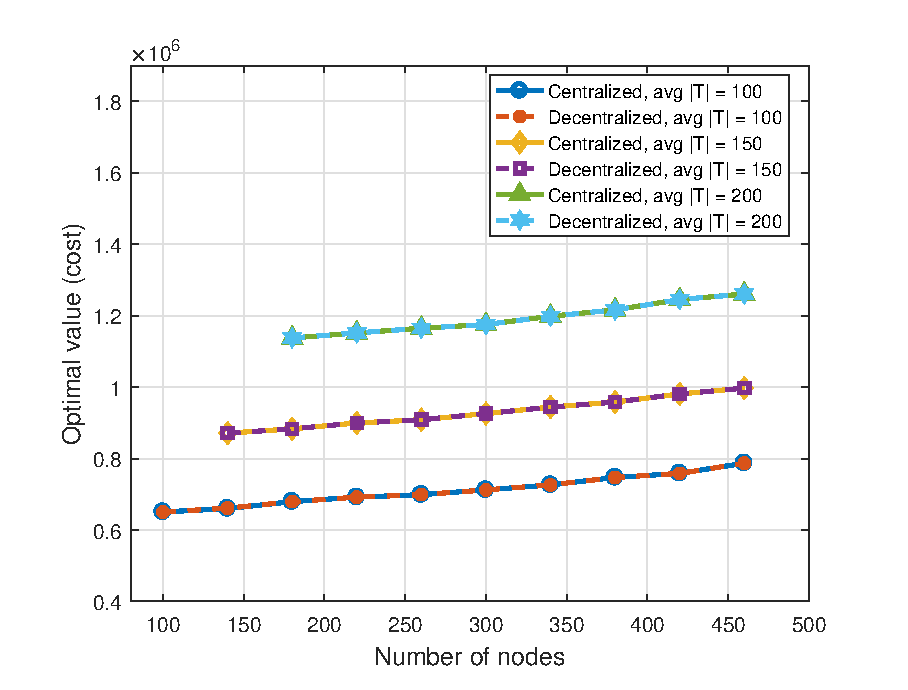
\includegraphics[width=12cm]{graphics/3-cent-decent/optimization_value_per_number_of_nodes}}
	\caption{مقدار تابع هدف(هزینه) دربرابر تعداد کل گره‌های موجود در شبکه برای دو روش متمرکز و غیرمتمرکز}
	\label{fig:optimization_value_per_number_of_nodes}
\end{figure}

    برای تاخیر مسیریاب‌ها فرض می‌کنیم که به صورت میانگین عبور بسته‌ها از مسیریاب‌های لایه 1، 2 میلی ثانیه، مسیریاب‌های لایه 2، 4 میلی ثانیه و مسیریاب‌های لایه 3، 10 میلی ثانیه طول می‌کشد.
\cref{fig:network} توپولوژی شبکه را که در شبیه‌سازی استفاده شده‌است نشان می‌دهد.

\begin{figure}[h!]
	\centerline{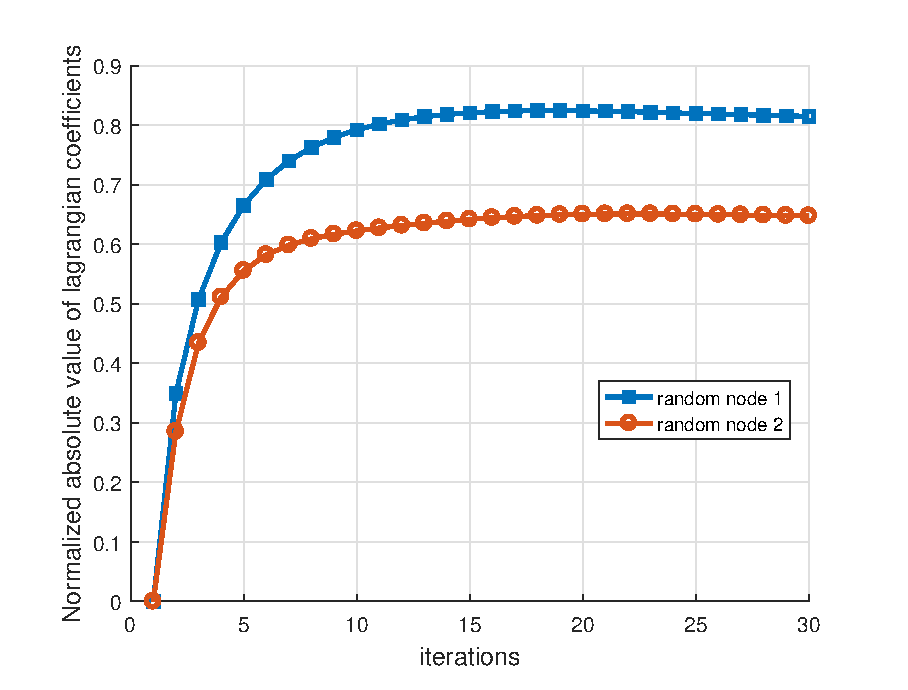
\includegraphics[width=12cm]{graphics/3-cent-decent/decentralized_lagrangian_coeffs_convergence}}
	\caption{نحوه‌ همگرا شدن اندازه ضرایب لاگرانژین در دو گره تصادفی در روش غیرمتمرکز}
	\label{fig:decentralized_lagrangian_coeffs_convergence}
\end{figure}

ظرفیت مربوط به هریک از گره‌ها به نجوی انتخاب شده است که بیشترین ظرفیت مربوط به گره‌های ابری و کمترین مربوط به گره‌های لبه باشد. که به ترتیب به نسبت اعداد 10، 9 و 8 درنظر گرفته شده است. حجم پردازنده مورد نیاز برای وظیفه‌ها نیز به صورت تصادفی اعداد حدود 40 واحد در نظر گرفته شده‌اند. حداقل زمان لازم جهت پردازش وظیفه‌ها به صورت تصادفی و حدود 15 میلی‌ثانیه فرض شده‌است. واحد قیمت پردازشی برای گره‌ها به صورتی در نظر گرفته شده است که ارزان‌ترین هزینه مربوط به گره‌های لایه ابری و گرانترین مربوط به گره‌‌های لایه لبه باشد، این اعداد به صورت تصادفی و به ترتیب به نسبت اعداد 1، 4 و 9 واحد در نظر گرفته شده‌است. نرخ پوآسون تولید وظیفه در گره‌های حسگری به صورت تصادفی و در حدود 50 واحد بر ثانیه برای هر وظیفه در هر گره حسگری درنظر گرفته شده‌است. 

\begin{figure}[h!]
	\centerline{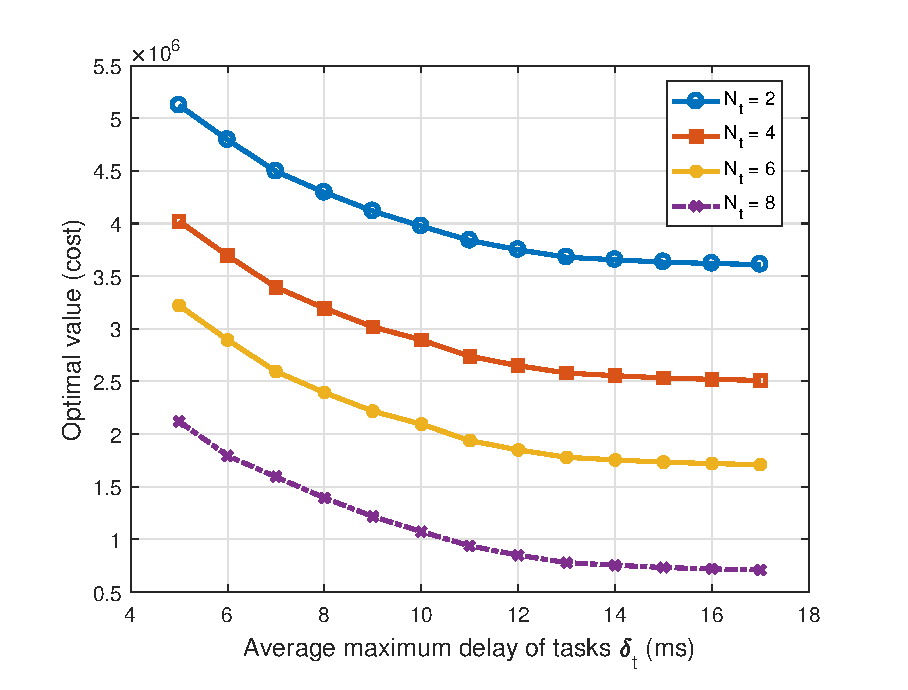
\includegraphics[width=12cm]{graphics/3-cent-decent/optimization_value_per_delay_for_dif_Nt}}
	\caption{مقدار تابع هدف(هزینه) دربرابر میانگین حداکثر تاخیر قابل قبول برای وظیفه‌ها $\delta_t$}
	\label{fig:optimization_value_per_delay_for_dif_Nt}
\end{figure}
	
	ابتدا لازم است که دقت دو روش متمرکز و غیرمتمرکز مقایسه شود. در \cref{fig:optimization_value_per_number_of_nodes} مقدار تابع هدف در این دو روش در برابر تعداد کل گره‌های موجود در شبکه از جمله گره‌های حسگری و گره‌های پردازشی دیده می‌شود. همانطور که دیده می‌شود این نمودار برای سه حالت مختلف از تعداد وظیفه‌ها رسم شده است و در هر سه حالت مقدار بهینه در روش متمرکز و غیرمتمرکز یکسان شده‌است. با افزایش تعداد کل وظیفه‌ها مقدار تابع هدف افزایش می‌یابد، همچنین با زیاد شدن کل گره‌های موجود در شبکه با فرض ثابت بودن تعداد وظیفه‌ها انتظار می‌رود که میزان تابع هدف تقریبا ثابت باشد، اما به دلیل اینکه با افزایش تعداد گره‌ها، تعداد گره‌های حسگری نیز افزایش می‌یابد، مقدار بهینه نیز اندکی افزایش می‌یابد. 

\begin{figure}[h!]
	\centerline{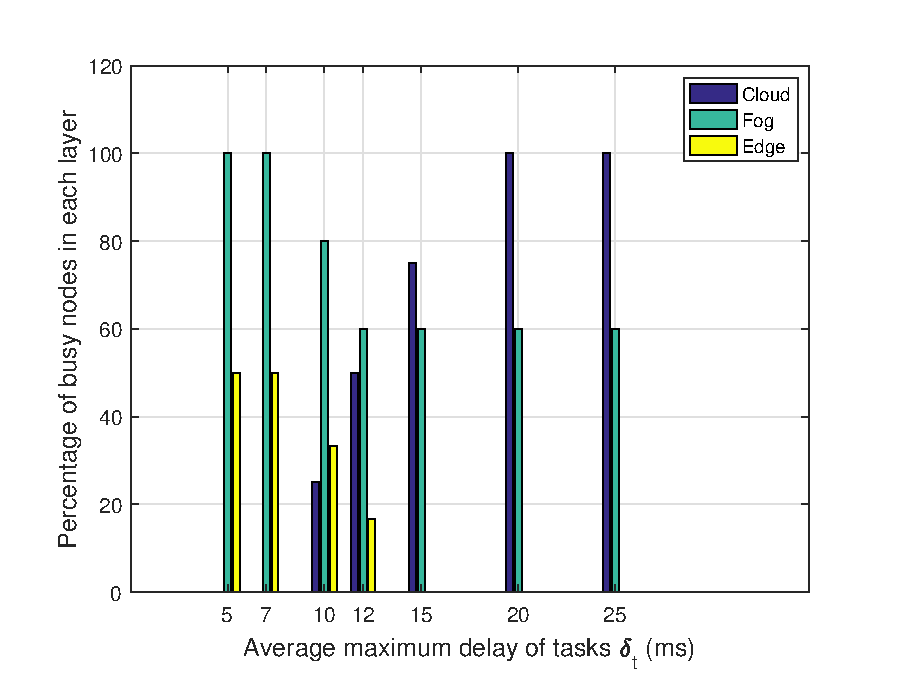
\includegraphics[width=12cm]{graphics/3-cent-decent/busynodes_per_delay}}
	\caption{درصد استفاده از گره‌های لایه‌های مختلف دربرابر میانگین حداکثر تاخیر قابل قبول برای وظیفه‌ها $\delta_t$}
	\label{fig:busynodes_per_delay}
\end{figure}

	درمورد روش غیرمتمرکز و نحوه‌ی همگرا شدن آن، دو گره به صورت تصادفی انتخاب شده‌است و در این دو گره مجموع اندازه‌ ضرایب لاگرانژ یعنی $\sqrt{|\eta_1|^2+|\eta_2|^2+|\nu_1|^2+|\nu_2|^2}$ به صورت یکه شده در طول زمان رسم شده است. در \cref{fig:decentralized_lagrangian_coeffs_convergence} می‌توانید این نتایج را ببینید.	

	در شبیه‌سازی بعدی تابع هدف براساس حداکثر تاخیرهای قابل قبول متفاوت برای وظیفه‌ها رسم شده است. با توجه به \cref{fig:optimization_value_per_delay_for_dif_Nt} می‌توان گفت که با افزایش میانگین حداکثر تاخیر قابل قبول برای وظیفه‌ها($\delta_t$) هزینه کل شبکه کاهش می‌یابد که دلیل این موضوع این است که استفاده از گره‌های ابری نسبت به گره‌های مه و لبه بیشتر می‌شود و از آنجایی که هزینه استفاده از گره‌های ابری کم‌تر است، هزینه کل شبکه کاهش می‌یابد. این نمودار برای چهار حالت مختلف از حداکثر تعداد قابل قبول برای تقسیم شدن وظیفه‌ها ($N_t$) رسم شده‌است. با توجه به \cref{fig:optimization_value_per_number_of_nodes} با کاهش $N_t$ این امکان کمتر می‌شود که وظیفه‌ها بین گره‌های مختلف شکسته شوند و هر وظیفه باید به صورت بخش‌های بزرگتری پردازش شود، درنتیجه استفاده از گره‌های مه و لبه بیشتر می‌شود و همین باعث می‌شود که هزینه کل شبکه بیشتر شود. 

\begin{figure}[h!]
	\centerline{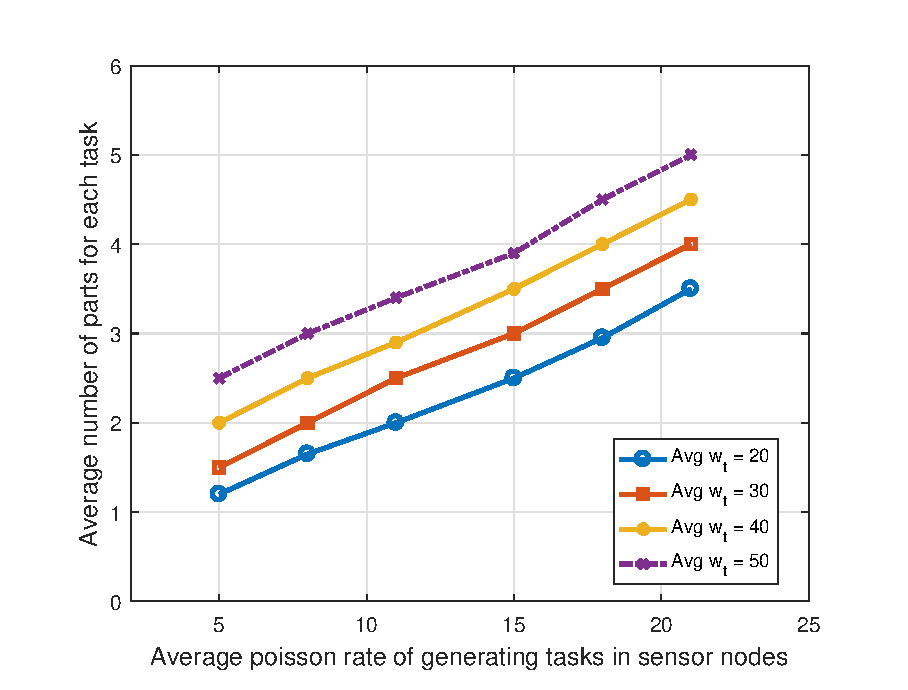
\includegraphics[width=12cm]{graphics/3-cent-decent/number_of_parts_per_task_generating_rate}}
	\caption{میانگین تعداد شکسته شدن وظیفه‌ها بین گره‌های مختلف دربرابر میانگین نرخ تولیدی وظیفه‌ها در گره‌های حسگری $\lambda_{t,s}$}
	\label{fig:number_of_parts_per_task_generating_rate}
\end{figure}

	در شبیه سازی بعدی میزان استفاده از گره‌های لایه‌های مختلف مورد تحلیل و بررسی قرار می‌گیرد. در \cref{fig:busynodes_per_delay} میانگین حداکثر تاخیر قابل قبول برای وظیفه‌ها در محور افقی قرار گرفته است و برای هر تاخیر، درصد استفاده از گره‌های هر لایه در محور عمودی نشان داده شده‌است. همانطور که دیده می‌شود با کاهش حداکثر میزان تاخیر قابل قبول لازم است که وظیفه‌ها بیشتر در سمت لبه پردازش شوند و این درصد استفاده از گره‌های این لایه را بیشتر می‌کند و بالعکس. 

	در آخرین شبیه‌سازی در این فصل قرار است که میزان شکسته‌شدن وظیفه‌ها بین گره‌های مختلف مورد بررسی قرار گیرد. برای این‌کار میزان نرخ تولید وظیفه‌ها در گره‌های حسگری تغییر کرده است و در هر مرحله میانگین تعداد شکسته شدن گره‌ها مورد بررسی قرار گرفته‌است. با توجه به \cref{fig:number_of_parts_per_task_generating_rate} می‌توان گفت که با افزایش میزان نرخ تولید وظیفه‌ها احتمال شکسته شدن وظیفه‌ها بین گره‌ها بیشتر می‌شود و میانگین تعداد تقسیم وظیفه‌ها افزایش می‌یابد. این نمودار برای میانگین حجم پردازشی وظیفه‌ها رسم شده‌است، که می‌توان گفت با افزایش میانگین حجم پردازشی، پردازش وظیفه‌ها سخت‌تر و درنتیجه میانگین تعداد تقسیم‌ها بیشتر می‌شود. 

	\section{جمع‌بندی و نتیجه‌گیری}
	در این فصل مدل سیستم برای مسئله تخصیص منابع پردازشی نوشته‌شد و مورد بررسی قرار گرفت. این مسئله غیرخطی بود که برای راحت‌تر شدن این مسئله خطی‌سازی شد. درادامه مسئله به کمک روش متمرکز حل شد و در نهایت یک الگوریتم برای حل مسئله به صورت غیرمتمرکز ارائه شد. هر دو روش گفته شده به جواب بهینه می‌رسند با این تفاوت که روش غیرمتمرکز در زمان خطی به جواب می‌رسد. 



